\documentclass{article}
\usepackage{amsmath,amssymb,amsfonts,amsthm, dsfont, color}
\usepackage{amsfonts}
\usepackage{tikz}
\usetikzlibrary{external}
\usetikzlibrary{shapes.misc, positioning}
\usetikzlibrary{decorations.pathreplacing}
\usetikzlibrary{arrows.meta, shapes,patterns.meta}

\tikzset{
  block/.style    = {draw, thick, rectangle, minimum width = 2em},
sblock/.style      = {draw, thick, rectangle, minimum height = 2em,
minimum width = 2em}, 
}
        
\definecolor{embed}{HTML}{AEF78E}
\definecolor{attn}{HTML}{f9e3ae}
\definecolor{ff}{HTML}{90F3FF}
\definecolor{lin}{HTML}{E15CEC}
\definecolor{mask1}{HTML}{4D4847}
\definecolor{mask2}{HTML}{30343F}
\definecolor{colour-zero}{HTML}{E83F6F}
\definecolor{colour-one}{HTML}{3f9fe8}
\definecolor{red}{rgb}{1.0, 0.0, 0.0}
\definecolor{lin}{HTML}{E15CEC}

\newcommand{\vect}[1]{\boldsymbol{#1}}
\newcommand{\bx}{\vect{x}}
\newcommand{\by}{\vect{y}}
\newcommand{\bz}{\vect{z}}
\newcommand{\bP}{\vect{P}}
\newcommand{\bbP}{\mathbb{P}}
\newcommand{\logit}{\mathrm{logit}}
\newcommand{\btheta}{\vect{\theta}}
\newcommand{\thetabar}{\bar{\btheta}}

\tikzexternalize

\begin{document}
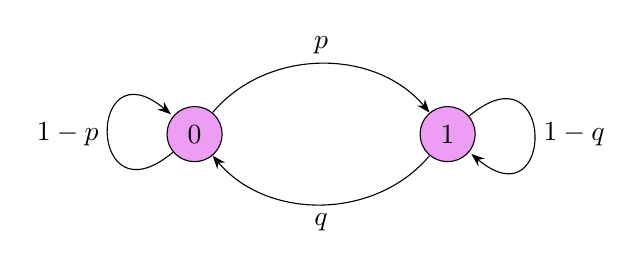
\begin{tikzpicture}[>=Stealth, node distance=2cm]
        % 0 and 1
        \node[circle,inner sep=0pt, minimum size=0.7cm,draw,fill=lin!60] (zero) {$0$};
        \node[circle,inner sep=0pt, minimum size=0.7cm,draw,right =2.5cm of zero,fill=lin!60] (one) {$1$};
        % arrows
        \draw [->] (zero) edge [bend left, out=50, in =130]  node[above] {$p$}   (one);
        \draw [->] (one)  edge [bend left, out=50, in =130]  node[below] {$q$}   (zero);
        \draw [->] (zero) edge [out=-140, in =140, loop]  node[left]  {$1-p$} (zero);
        \draw [->] (one)  edge [in=-40, out=40, loop] node[right] {$1-q$} (one);
        % find midpoint
        \path (zero) -- (one) node[pos=0.5] (midup) {};
    \end{tikzpicture}
\end{document}